\chapter{METHODOLOGY}
In this chapter, the methodology is detailed as follows.  
First, we describe the architecture of the model.  
Second, we explain all pre-training loss functions used in this experiment.  
Third, the details of \acrshort{pos} tagging are provided.  
Fourth, we outline the datasets used in this experiment.  
Lastly, we provide details on the visual question answering setup.  

\begin{figure}[h]
    \caption{Overall methodology}
    \label{fig:overview}
    Pre-training the model with a \acrshort{mlm} task by masking tokens based on the \acrshort{pos} in the image captions.
    \begin{center}
        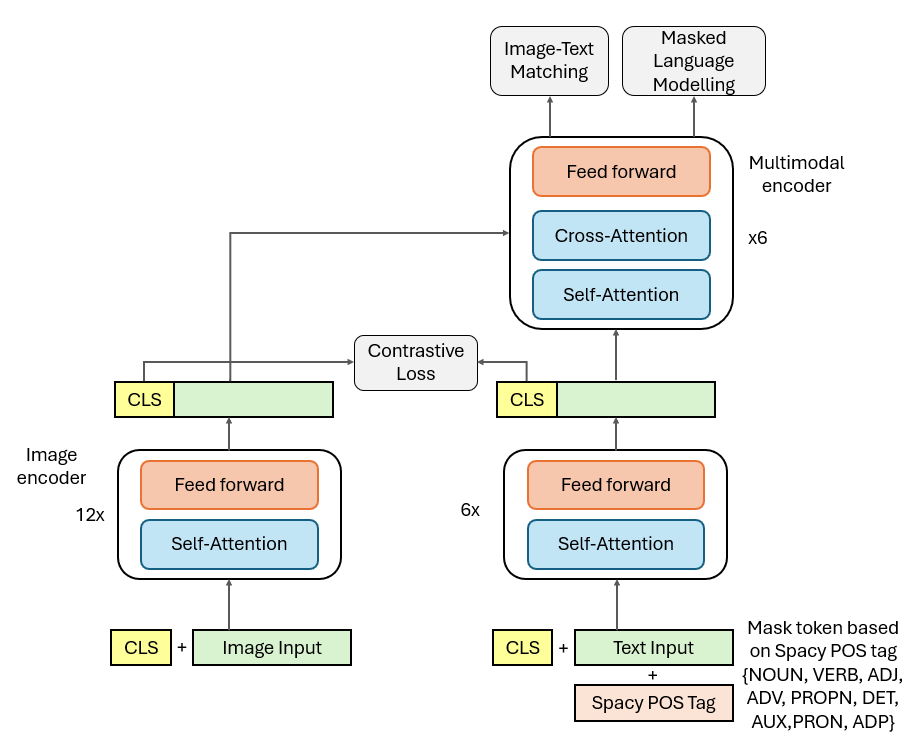
\includegraphics[width=0.8\textwidth]{Images/overview.png}
    \end{center}
    \small
\end{figure}

\section{Model architecture}
As shown in Figure \ref{fig:overview}, our model includes three main components: an image encoder, a text encoder, and a multimodal encoder.  
The first component is the image encoder, for which we use ViT \cite{vit}, modified following \cite{clip}, as the image encoder in this experiment.  
The second component is the text encoder, which employs a transformer architecture as BERT \cite{bert} to encode image captions with BERT tokenizer for tokenization.  
The final component is the multimodal encoder, where \acrshort{vl} interactions occur.  

Given a training dataset \(D\) consisting of image-text pairs \((I_i, T_i) \in D\), where \(I_i\) is the image and \(T_i\) is the image caption of the \(i\)-th image, each image is first encoded as a sequence of tokens \(\{v_{cls}, v_1, \dots, v_n\}\) using ViT \cite{vit}.  
Here, \(v_{cls}\) represents the embedding of the [CLS] token prepended to the image patch sequence.  
In this experiment, the image encoder was initialized with ViT-B-32 pre-trained on ImageNet-21K \cite{imagenet}.  
Next, we use a 6-layer transformer, randomly initialized, to encode the image caption \(T_i\) into text embeddings \(\{w_{cls}, w_1, \dots, w_n\}\), where \(w_{cls}\) is the embedding of the [CLS] token.  
Finally, both text and image encodings are passed through the multimodal encoder to fuse both inputs, producing multimodal encodings.  
For the multimodal encoder, a cross-attention layer is used, where both keys and values are the image encodings, and the text encoding serves as the query in the cross-attention layer.  


% Cross Attention using Image = K, V Text as a query.
% Thought: The image encoder choice can be change based on training speec.
\section{Pre-training Objectives}
In this work, we pre-train our model with three objectives: \acrfull{mlm}, \acrfull{itc} and \acrfull{itm}.
\subsection{Mask Language Modelling}
Typically, a percentage of tokens \(\{w_1, \dots, w_T\}\) are replaced with a special [MASK] token to create a masked caption \(T^{\text{mask}}\).  
However, in this work, the masked tokens were selected based on \acrshort{pos} type instead of randomly masking.  
The model trained to predict the original tokens at the masked positions, conditioned on both the unmasked tokens in \(T^{\text{mask}}\) and the visual features of \(I\) as \(p^{\text{mask}}(I, T^{\text{mask}})\).  
Let \(y^{\text{mask}}\) be a one-hot vector representing the ground-truth vocabulary for the masked token, where the masked token has a probability of 1.  
The model’s objective is to minimize the cross-entropy \(\mathbf{H}\), given by:  
\[
    \mathcal{L}_{\text{MLM}} = \mathbf{H}(y^{\text{mask}}, p^{\text{mask}}(I, T^{\text{mask}})))
\]
For the masking ratio, each POS token is masked with either a 70 percent or 100 percent probability.
In this work, random token masking was also tested with a masking ratio of 15 percent.

\subsection{Image-Text Contrastive Learning}
To improve each unimodal encoder's representation, we used \acrlong{itc} to improve alignment of each modality.  
\acrshort{itc} aims to improve alignment by maximizing the similarity score of image and text from the same pair with the score function \(s(I, T) = v_{cls}^\top w_{cls}\), and minimizing the similarity score of image and text not from its pair.  
We then calculate the softmax-normalized similarity score for each image to any text and each text to any image, identified as image-to-text \(p^{i2t} \in \mathbb{R}^{M}\) and text-to-image \(p^{t2i} \in \mathbb{R}^{M}\) scores as:  
\[
    p^{i2t}_i(I) = \frac{ \exp{(s(I,T_i))/\tau} }{ \sum_{m=1}^{M}\exp{(s(I,T_m)/\tau} }, \quad p^{t2i}_i(T) = \frac{ \exp{(s(T,I_i))/\tau} }{ \sum_{m=1}^{M}\exp{(s(T,I_m)/\tau} }
\]
where \(\tau\) is a learnable temperature parameter.  
Let \( y^{i2t}(I) \in \{0,1\}^M \) and \( y^{t2i}(T) \in \{0,1\}^M \) be a ground truth with probability of 1 at a position of the same pair, and probability of 0 on the other hand.  
The \acrshort{itc} loss is calculated as cross-entropy \(\mathbf{H}\) between \(p\) and \(y\):  
\[
    \mathcal{L}_{\text{ITC}} = \frac{1}{2}(\mathbf{H}(y^{i2t},p^{i2t}) + \mathbf{H}(y^{t2i},p^{t2i}))
\]
\subsection{Image-Text Matching}
To further improve multimodal alignment in the \acrshort{vl} model, \acrlong{itm} was employed to enhance alignment.  
The model is trained to predict whether an image and caption are from the same pair.  
A fully connected layer, followed by a softmax function, is added over the model.  
This layer takes the [CLS] embedding from the multimodal encoding as input to predict whether the pair is positive (matched) or negative (unmatched).  

The loss function for \acrshort{itm}, using cross-entropy loss, is defined as:  
\[
    \mathcal{L}_{\text{ITM}} = \mathbf{H}(y^{\text{itm}}, p^{\text{itm}}(I, T)),
\]
where \(y^{\text{itm}}\) is a one-hot ground-truth label, and \(p^{\text{itm}}(I, T)\) is the predicted class probability.

The full pre-training objective of our work can be written as:
\[
    \mathcal{L} = \mathcal{L}_{\text{MLM}} + \mathcal{L}_{\text{ITC}} + \mathcal{L}_{\text{ITM}}
\]

\section{Part Of Speech Masking}
For each image caption, each token was classified into \acrshort{pos} categories for masking.  
We used POS-tagging tools SpaCy\footnote{POS-tagging tool SpaCy: https://spacy.io/} to classify each word into \acrshort{pos} classes based on the Universal POS tag set\footnote{Universal POS tag set: https://universaldependencies.org/u/pos/}.
In this work, we modified the BERT tokenizer to integrate with SpaCy by using the Tokenizations\footnote{Tokenizations alignment library tool: https://github.com/explosion/tokenizations} tool to align BERT token IDs with SpaCy tokens IDs.

In this experiment, we explored the effect of each \acrshort{pos} on \acrshort{vl} learning in terms of performance, and training loss.  
For the main experiment, each token was assigned to one of nine \acrshort{pos} categories: NOUN (nouns), VERB (verbs), ADJ (adjectives), ADV (adverbs), PROPN (proper nouns), DET (determiners), AUX (auxiliaries), PRON (pronouns), and ADP (adpositions), and masked with a 70\% probability.
For evaluation, these \acrshort{pos} were further classified as functional (determiners, auxiliaries, pronouns, adpositions) or non-functional (nouns, verbs, adjectives, adverbs, proper nouns).
For the 100 percent masking setting, where all tokens corresponding to a specific \acrshort{pos} are masked, we conducted experiments on non-functional parts of speech.

\section{Pre-Training Dataset}
We pre-trained the model on the Conceptual Captions dataset \cite{conceptual-caption} and the MSCOCO dataset, totaling 2.4 million image-text pairs.
In Conceptual Captions dataset, an automated process was used to select, filter, and refine these image-caption pairs to ensure they are clear, informative, and suitable for effective model training.

% \section{Continue Training}
% In this experiment, we explored the effect of each POS in the continue training situation, where the amount of dataset is limited, and the domain is difference from the pre-training dataset.
% We trained each model on difference categories of \acrshort{pos} with every datasets, including GoodNews \cite{goodnew}, RSICD \cite{rsicd}, and Sketchy Scene \cite{sketchy-scene}
% The model was initialized with ALBEF pre-training weights. 
% The GoodNews dataset is an image-text pair dataset gather from New York Times.
% This dataset have total image-text pairs of 466,000 pairs, randomly splited into 424,000 for training, 18,000 for validation, and 23,000 for testing.
% For RSICD, the dataset include a remote sensing image in total of 10,921 images with 5 captions per image.
% The Sketchy Scene dataset include total of 1,000 image-text pairs.

\section{Evaluation}
In this work, we evaluated each model trained with different types of \acrshort{pos} masking through image-text retrieval, image-text matching, and visual question answering tasks.  
Details of the evaluation methods and datasets used in these tasks are provided in this section.  

\subsection{Image-Text Retrieval}
For the image-text retrieval, the model was tested by performing zero-shot evaluations on the Flickr30K \cite{flickr30k} dataset for both \acrfull{ir} and \acrfull{tr}.  
The Flickr30K dataset is used to assess the model's overall performance in retrieval tasks.
This setup allowed us to analyze how different \acrshort{pos} masking strategies affect the model's retrieval performance and the alignment between visual and textual representations.  

\subsection{Image-Text Matching}
As demonstrated by \citeA{rf-curriculum-masking}, the results suggest that masking strategies impact a model’s ability to understand attributes, relationships, and word order.  
In this work, we benchmarked each pre-trained model with specific \acrshort{pos} masking against VALSE benchmark \cite{valse}.  
For the VALSE dataset, this benchmark categorizes each image-text sample into different linguistic phenomena as showed in Table \ref{tab:valse_detail}, including six distinct types: existence, plurality, counting, relation, action, and coreference.  
Each image caption in the VALSE dataset also includes a "Foil" version, where words related to each caption category are modified.  
This task is a classification task, where the model has to predict the correct caption for each image.
We evaluated the model in a zero-shot manner by reusing the \acrshort{itm} head as a classifier.
Evaluating models against this benchmark provides valuable insights into their semantic and contextual understanding of vision and language modality.  

\begin{table}[h]
    \caption{VALSE dataset task explanations.}
    \label{tab:valse_detail}
    \centering
    \begin{tabular}{|l|p{4cm}|p{5cm}|}
        \hline
        \textbf{VALSE Task} & \textbf{Test} & \textbf{Example} \\ \hline
        Existence Quantifier & Detect object presence or absence & ``A cat on bed'' vs. ``A dog on bed'' \\ \hline
        Plurality Number & Singular vs. plural & ``One flower'' vs. ``Some flowers'' \\ \hline
        Counting Balanced & Count with equal samples per class & 3 apples vs. 5 apples \\ \hline
        Counting Adversarial & Test for small-number bias & counts $\ge$ 4 vs counts 0–3 \\ \hline
        Counting Small Numbers & Count small numbers only & counts $<$ 4 \\ \hline
        Spatial Relation & Understand positions & ``Book on table'' vs. ``Book under table'' \\ \hline
        Action Replacement & Correct action & ``Holding ball'' vs. ``Throwing ball'' \\ \hline
        Actant Swap & Correct roles & ``Boy chases dog'' vs. ``Dog chases boy'' \\ \hline
        Coreference Standard & Pronoun–Entity Relation Understanding (from test set) & ``Woman talks to girl. She smiles.'' \\ \hline
        Coreference Hard & Coreference Standard (from val set) & ``Boy hugs dog. He is happy.'' \\ \hline
        Foil-COCO & Spot small caption error & Correct vs. nearly identical with one mistake \\ \hline
    \end{tabular}
\end{table}

\begin{figure}[h]
    \caption{Visual question answering model architecture}
    \label{fig:vqa}
    \begin{center}
        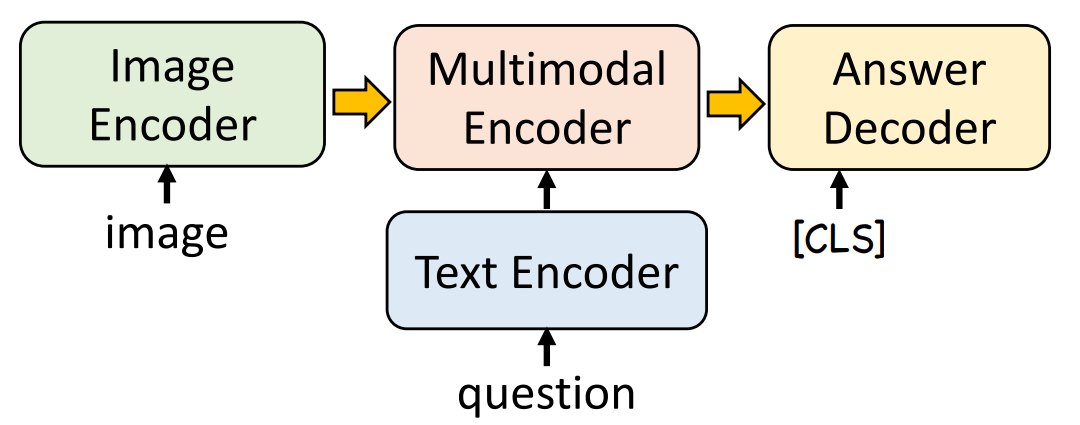
\includegraphics[width=0.6\textwidth]{Images/vqa_method.png}
    \end{center}
    \small
\end{figure}

\subsection{Visual Question Answering}
In this work, the \acrfull{vqa} task was treated as a classification task.
A classification head was appended to generate the answer, as shown in Figure \ref{fig:vqa}.
The benchmark dataset for the \acrshort{vqa} task is the VQA2.0 dataset \cite{vqa2}, which is constructed using images from COCO \cite{mscoco}.  
This dataset includes 83,000 images for training, 41,000 for validation, and 81,000 for testing.  
We further train our model using the VQA2.0 training set.

\section{Training}
The model was pre-trained on a machine equipped with four NVIDIA A100 GPUs.
The pre-training of the model was conducted using a batch size of 64 with 10 epochs.
We used the AdamW optimizer with an initial learning rate of \(1 \times 10^{-4}\) and a weight decay of 0.02 to help regularize the training process.
A cosine learning rate scheduler was applied, with the learning rate gradually increasing from a warm-up value of \(1 \times 10^{-5}\) during the first 5 epochs, before decaying towards a minimum learning rate of \(1 \times 10^{-5}\) by the end of training.

For the VQA task, the model was trained with a batch size of 32 on the same machine as pre-training.
We used the AdamW optimizer with a learning rate of \(2 \times 10^{-5}\) and a weight decay of 0.02.
A cosine learning rate scheduler was applied over 8 epochs, with a warm-up phase of 1 epoch starting at a learning rate of \(1 \times 10^{-5}\), and decaying to a minimum of \(1 \times 10^{-6}\).